
\clearpage{}
\section{Benchmarks}
\label{section:Benchmarks}
In this section we present several programs where the baseline array representation worsened the asymptotic complexity of the vectorised program. All benchmarks were taken on an Intel i7 QuadCore / 8GB desktop machine. We have opted to present data for the program running in single threaded mode only. We have not finished adapting our parallel stream fusion framework to the new array representation, so parallel speedup is currently dominated by the creation of intermediate arrays such as the ``boring'' fields described in \S\ref{section:Promotion} and \S\ref{section:Pragmatics}. However, all of the underling primitives we use operate on bulk arrays and are amenable to parallelisation. 


% -- SMVM ---------------------------------------------------------------------
\subsection{Sparse Matrix-Vector Multiplication}
This program multiples a sparse matrix by a dense vector and is discussed in \cite{Leshchinskiy:higher-order-ndp}. The matrix is represented as an array of rows, where each row is an pair of a column index and the @Double@ value in that column.
%
\begin{small}
\begin{code}
smvm :: [:[:(Int, Double):]:] -> [:Double:] -> [:Double:]
smvm matrix vector
 = let term (ix, coeff) = coeff * (vector ! ix)
       sumRow row       = sumP (mapP term row)
   in  mapP sumRow matrix
\end{code}
\end{small}
%
As @vector@ is free in the definition of @term@, with the old array representation it would be copied once for every non-zero element of the matrix. With the new array representation the vector is not copied and it runs with the same asymptotic complexity as an unvectorised reference implementation written with the @Data.Vector@ package. The @Data.Vector@ version is currently faster than with our new representation because stream fusion \cite{Coutts:streamfusion} does a better job at eliminating intermediate values.


% -- TreeLookup ---------------------------------------------------------------
\subsection{Tree Lookup}
\label{section:TreeLookup}
The following microbenchmark exposes the replicate problem in sharp relief. It performs a divide-and-conquer of an @indices@ array, while referring to a top level @table@. In the base case, a single index is used to access the top-level table, and the table is rebuilt during the return calls. 
%
\begin{small}
\begin{code}
 treeLookup :: [:Int:] -> [:Int:] -> [:Int:]
 treeLookup table indices
   | lengthP indices == 1 = [:table !: (indices !: 0):]
   | otherwise
   = let half = lengthP indices `div` 2
         s1   = sliceP 0    half indices
         s2   = sliceP half half indices           
     in concatP (mapP (treeLookup table) [: s1, s2 :])
\end{code}
\end{small}
%
As @table@ is partially applied to @treeLookup@, with the baseline representation the entire @table@ is copied once for every element of @indices@. In the vectorised version the call to @replicate@ cannot be eliminated with the rewrite rules discussed in \S\ref{section:RewriteRules}, because the producer and consumer of the replicated array are in different recursive calls. With our new array representation, the sharing is managed by our @segmap@ and the elements of @table@ are not copied.


% -- Barnes-Hutt --------------------------------------------------------------
\subsection{Barnes-Hut}
The Barnes-Hut algorithm performs a two dimensional gravitation simulation of many massive bodies. At each time step, the algorithm builds a quad-tree to partition the space the bodies lie in, and computes the centroid of all bodies in each branch. The tree is then used to compute the force between each body and all the others, approximating the force between distant bodies by using the centroids. Whereas a naive algorithm would use work $O(n^2)$ in the number of bodies, the Barnes-Hut approximation is $O(n . log~ n)$.

With the baseline array representation, the copying replication problem appears at the very top level. Once we have built the quad-tree, we use it to compute the force on each body. \eject

\noindent
This is done by the following function:
\begin{small}
\begin{code}
 calcAccels :: Double -> Box -> [:MassPoint:] -> [:Accel:]
 calcAccels epsilon boundingBox points
  = mapP (\m -> calcAccel epsilon m tree) points
  where tree = buildTree boundingBox points
\end{code}
\end{small}
As @tree@ is free in the closure passed to @mapP@, it is copied once for every body. As before, with the new array representation the tree is not copied and the program runs with the same asymptotic complexity as an unvectorised reference implementation written with the @Data.Vector@ package.


% -----------------------------------------------------------------------------
\begin{figure}
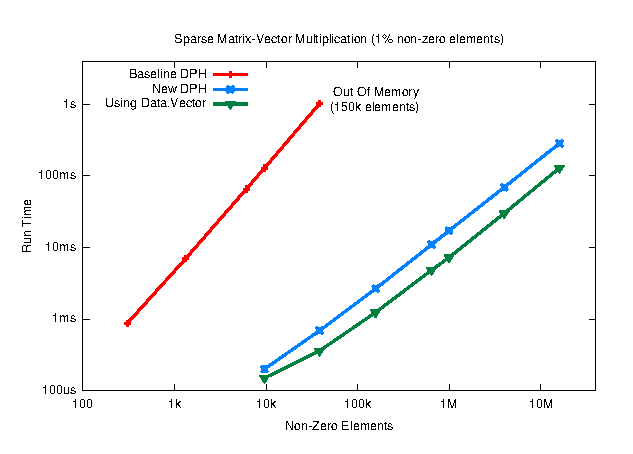
\includegraphics[scale=0.8]{data/smvm}
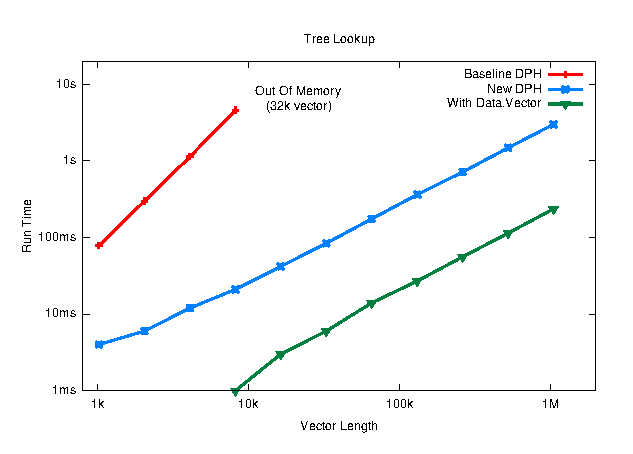
\includegraphics[scale=0.8]{data/indices}
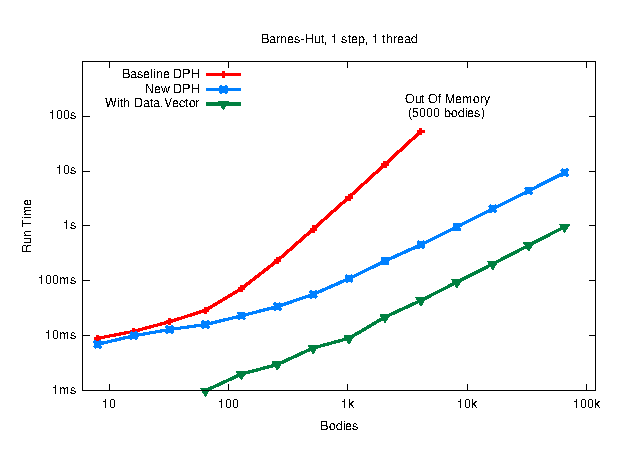
\includegraphics[scale=0.8]{data/nbody}
\caption{Benchmark Runtime Performance}
\label{figure:Benchmarks}
\end{figure}

When divide and conquer algorithms such as \mbox{Barnes-Hut} are vectorised, the resulting code increases the nesting level of the source array during the division phase (on the way down) and concatenates the result on the way back up. We refer to such algorithms as \emph{dynamically nested} for this reason. As discussed in \S\ref{section:ConcatUnconcat}, @concat@ normalises the array representation, so the program effectively switches between the old baseline representation and our new scattered representation as it runs.
